\documentclass[a4paper, 11pt]{article}

\usepackage[swedish]{babel}
\usepackage[utf8]{inputenc}
\usepackage[T1]{fontenc}
\usepackage{lmodern}

\usepackage{tikz}

\tikzset{
  excl/.style = {circle, draw=black, inner sep=0pt, minimum size=4pt}
}

\tikzset{
  incl/.style = {circle, draw=black, fill=black, inner sep=0pt, minimum size=4pt}
}


\usepackage{pgfplots}


\usepackage{graphicx}
\usepackage{caption}
\usepackage{subcaption}

\usepackage{enumitem}

\usepackage{multicol}

\usepackage{amsmath}


\begin{document}

\title{
    \textbf{MM2001: Inläming 1}
}
\author{Johan Montelius}
\date{HT 2026}

\maketitle

\section*{i)}

Betrakta funktionen: $f(x) = -sin(3x) + cos(3x$).
\begin{enumerate}[label=\alph*)]
  \item Skriv om funktionen $f(x)$ på formen $A\, sin(kx + \delta)$.
  \item Lös ekvationen  $f(x) = 1$.
\end{enumerate}

\subsection*{a)}

\noindent Vi kan använda oss av {\em hjälpvinkelmetoden}. Skriver vi funktionen
på formen:
$$ a\, sin(n) + b\, cos(n)$$ så kan vi skriva om den som:
$$ \sigma\, sin(n + \delta) $$
där $\sigma = \sqrt{a^2 + b^2}$ och $a/\sigma = cos(\delta)$.

\vspace{5pt} Givet funktionen $f(x)$ har vi att $a = -1$, $b = 1$ och
$n = 3x$. Detta ger oss $\sigma = 1$ och $-1 = cos(\delta)$ vilket ger
oss $\delta = \pi$. Vi har då:

\begin{align*}
 f(x)  &=\; sin(3x + \pi) &\; \\
       &=\; -sin(3x) &\; \text{ ty\ } sin(v) = -sin(v + \pi)\\
\end{align*}


\subsection*{b)}

\begin{align*}
  -sin(3x) + cos(3x) &=\;  1 &\\
  -sin(3x) &=\; 1 &\; \text{enligt lösningen i a) ovan}\\
  3x &=\; 3\pi/2 + 2\pi n &\\
  x &=\; \pi/2 + (2/3)\pi n &\\
\end{align*}

\section*{ii)}

Kolla hjälpvinkelmetoden och harmoniska svängningar i kursboken PB1
(Persson-Böiers). Där finns begreppen amplitud och period.

\begin{enumerate}[label=\alph*]
\item På vilken sida i boken har du hittat dessa?
\item Ange både amplituden och perioden för funktionen $f$ i (i).
\end{enumerate}

\subsection*{a)}  Sindan 110.

\subsection*{b)}  Amplituden = -1 och perioden = $2\pi / 3$


\section*{iii)} Skissa (utan datorhjälp) grafen för funktionen $f$ i (i) utifrån grafen för funktionen $g(x) := sin 3x$.

Svar i Fig \ref{fig:iii}. 

\begin{figure}
  \center
  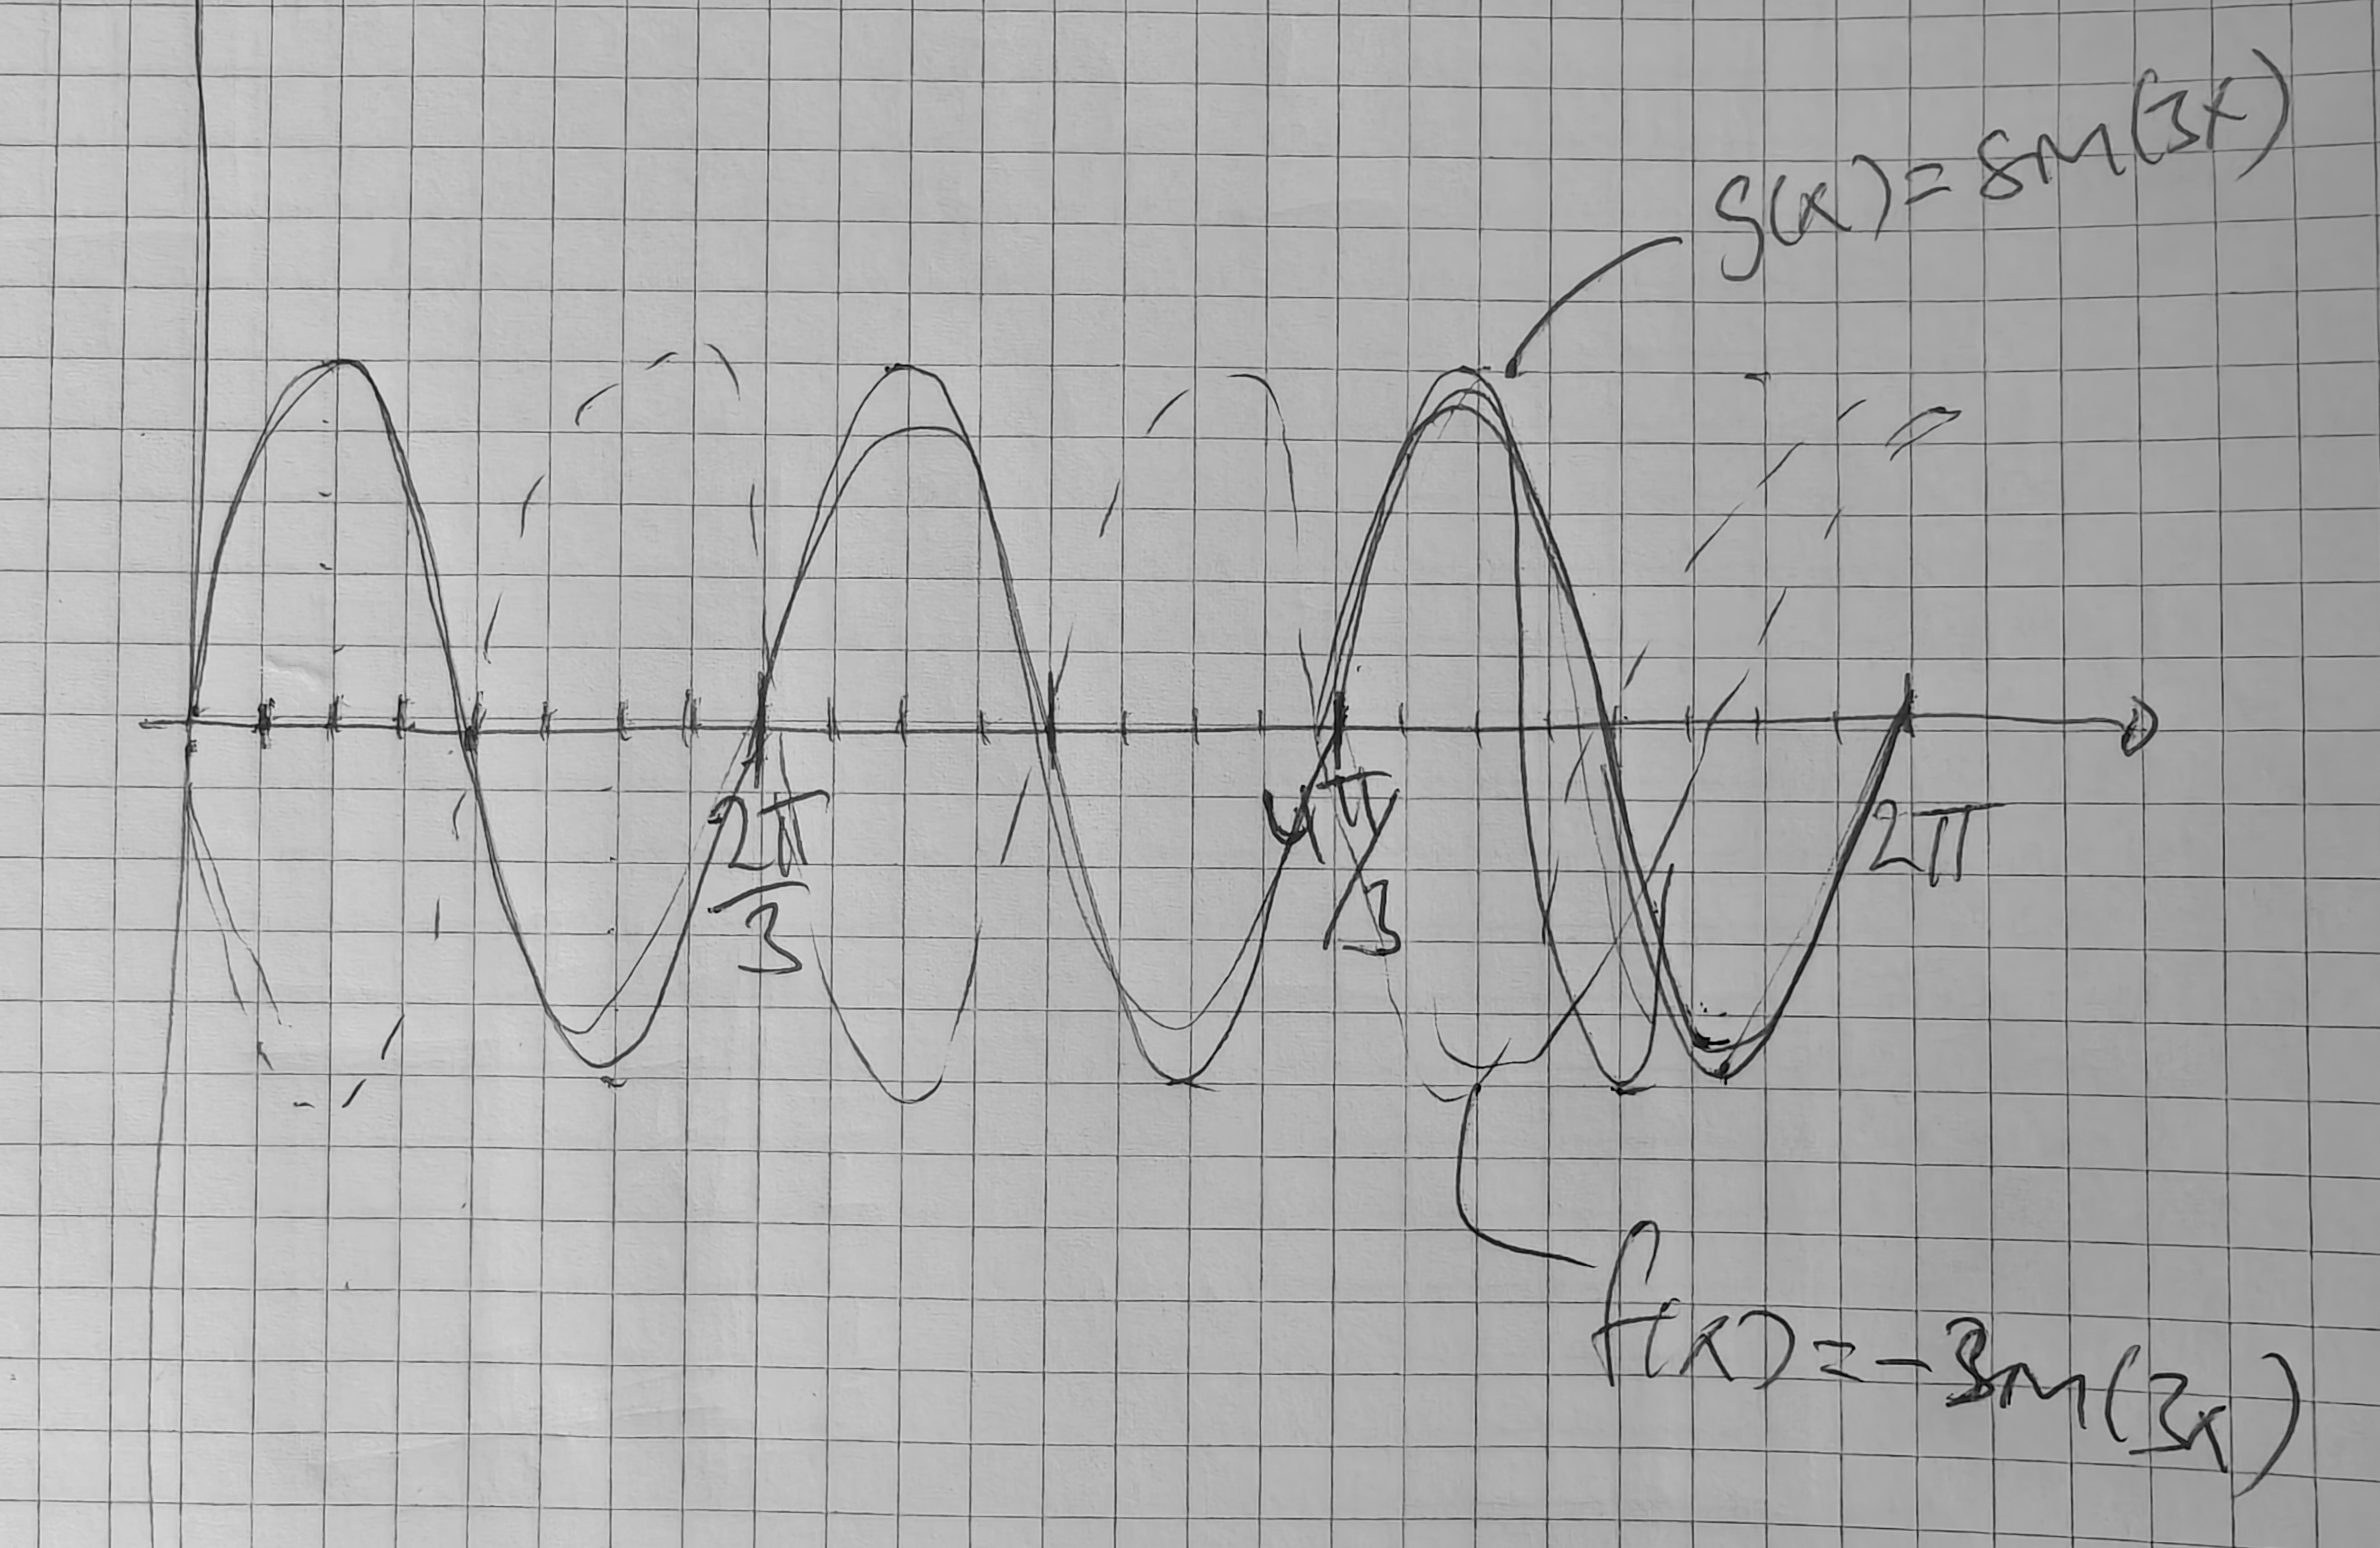
\includegraphics[scale=0.1]{sin-1.png}
  \caption{Svar på fråga iii) - skissa grafen till f(x) utifrån g(x) = sin(3x).}
  \label{fig:iii}
\end{figure}

\end{document}


